\chapter{Appendix}

\section{Detector Signatures of Different Neutrino Flavors}
\begin{figure}
  \centering
  \begin{subfigure}{0.3\textwidth}
    \centering
    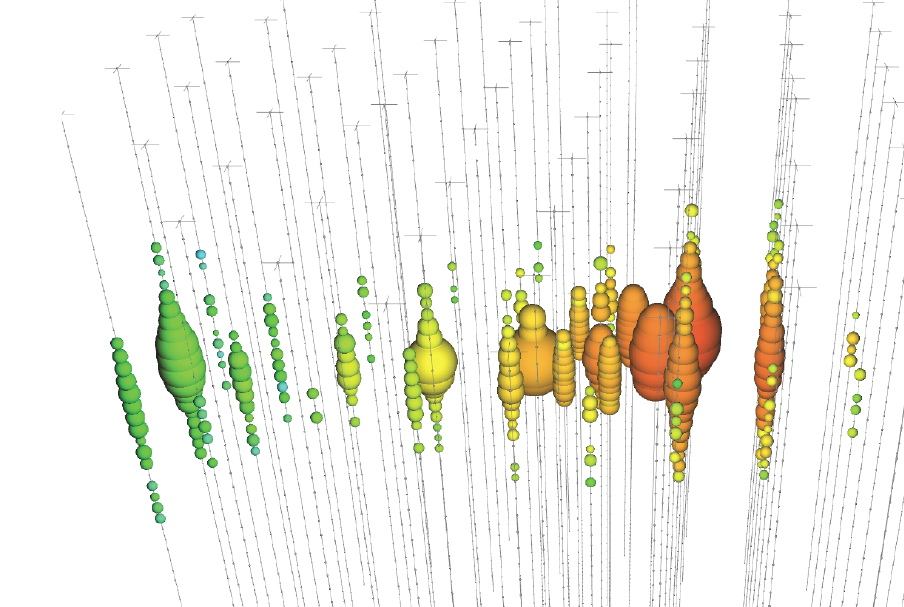
\includegraphics[width=\textwidth]{content/img/signatures/track.png}
    \caption{
        Track / $\nu_\mu$
    }
  \end{subfigure}
  \begin{subfigure}{0.3\textwidth}
    \centering
    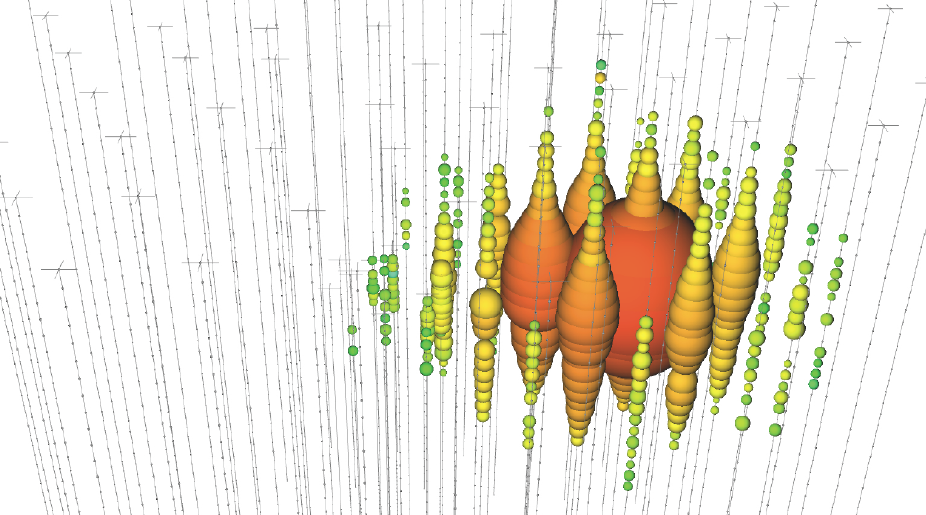
\includegraphics[width=\textwidth]{content/img/signatures/cascade.png}
    \caption{
        Cascade / $\nu_e$
    }
  \end{subfigure}
  \begin{subfigure}{0.3\textwidth}
    \centering
    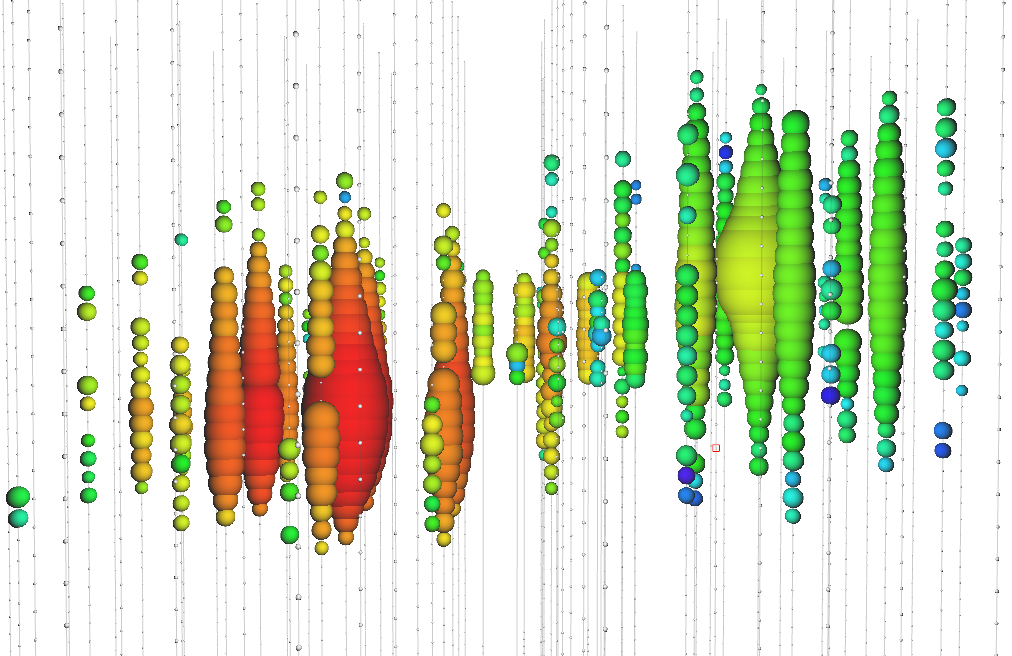
\includegraphics[width=\textwidth]{content/img/signatures/double_bang.png}
    \caption{
        Double bang / $\nu_\tau$
    }
  \end{subfigure}
  \caption{
    Shapes of the Cherenkov light produced by neutrinos of different flavors.
    The coloring of the \acp{DOM} indicates the time of the interaction,
    with red being the earliest and blue being the latest.
    \cite{kowalski2017} % CC-BY 3.0
  }
  \label{fig:img:icecube:interactions}
\end{figure}


\clearpage
\section{\dseaplustitle{}: Complete Algorithm} \label{sec:alg:dseaplus}
\begin{algorithm}
  \caption{
    The \dseaplus{} algorithm with reweighting of training examples and adjustable stepsize. \cite{dsea_mirko}
    \todo[inline]{
      This is taken 1:1 from Mirko's thesis.
      I didn't quite get @Karolin's feedback on this:
      Should I remove it?
      }
    }
  \label{alg:dseaplus}
  \begin{algorithmic}
    \newcommand{\f}{\mathbf{f}}
    \newcommand{\hatf}{\hat{\mathbf{f}}}
    \newcommand{\x}{\mathbf{x}}

    \Require{
      \\
      Observed data set $\mathcal{D}_\text{obs} = \{ \x_n \in \mathcal{X} : 1 \leq n \leq N \}$ \\
      Training data set $\mathcal{D}_\text{test} = \{ (\x_n, y_n) \in \mathcal{X} \times \{1,\ldots,I\} : 1 \leq n \leq N' \}$ \\
      $\tau \geq 0$, regularization strength employed in the stepsize adaptation (default: \num{0}) \\
      $\epsilon > 0$, the minimal $\chi_\text{Sym}^2$ distance between subsequent iterations (default: \num{E-6}) \\
      Prior density $\hatf^{(0)}$ (default: $\hatf_i^{(0)} = \frac{1}{I} \forall 1 \leq j \leq J$)
    }
    \Ensure Estimated target density $\hatf \in \mathbb{R}^I$
    \State $k \gets 0$
    \Repeat
      \State $k \gets k-1$\;
      \State $\forall 1 \leq n \leq N': w_n^{(k)} \gets \hatf_{i (n)}^{(k-1)} / \f_{i (n)}^t$\;
      \State Infer $\mathcal{M}$ from $\mathcal{D}_\text{train}$ weighted by $w_n^{(k)+}$\;
      \State $\forall 1 \leq i \leq I: p_i^{(k)} \gets \frac{1}{N} \sum_{n=1}^N c_{\mathcal{M}}(i|\x_n) - \hatf^{(k-1)}$\;
      \State $\alpha_{\textsc{Run}}^{(k)} \gets \operatorname{argmin}_{\alpha \geq 0} \ell_r(\hatf^{(k-1)} + \alpha p^{(k)})$\;
      \State $\hatf_i^{(k)+} \gets \hatf^{(k-1)} + \alpha_{\textsc{Run}}^{(k)} \cdot p^{(k)}$\;
    \Until $\chi_\text{Sym}^2(\hatf^{(k)}, \hatf^{(k-1)}) \leq \epsilon$\; \\
    \Return $\hatf \gets \hatf^{(k)}$
  \end{algorithmic}
\end{algorithm}



\clearpage
\section{From Threshold to Per-Class Probabilities}
\label{sec:appendix:corn_probas}
Given four ranks with indices $q \in \{1, 2, 3, 4\}$,
\corn{}'s output layer has three neurons, which
  – after applying sigmoid and a cumulative product –
yield three threshold probabilities:
	$P[q>1]$,
	$P[q>2]$ and
	$P[q>3]$.
The goal is to calculate the probability of each class $q$,
i.e. $P[q=1]$, $P[q=2]$, $P[q=3]$ and $P[q=4]$.

% The solution explicitly requires the assumption that…
Using $q \in \{1, 2, 3, 4\}$,
the following equations hold:
\begin{align*}
  P[q=1] &= \neg P[q>1] = 1 - P[q>1] \\
  \\
  P[q=2] &= \neg P[q≠2] \\
  &= \neg(P[q<2] \lor P[q>2]) \\
  &= 1 - ((1 - P[q>1]) + P[q>2]) \\
  &= P[q>1] - P[q>2] \\
  \\
  P[q=3] &= \neg P[q≠3] \\
  &= \neg(P[q<3] \lor P[q>3]) \\
  &= 1 - ((1 - P[q>2]) + P[q>3]) \\
  &= P[q>2] - P[q>3] \\
  \\
  P[q=4] &= P[q>3] % NOTE: no “.” (@Karolin)
\end{align*}

The same principle can be applied to any number of classes.


\clearpage
\section{Monte Carlo Dataset}
\begin{figure}
  \centering
  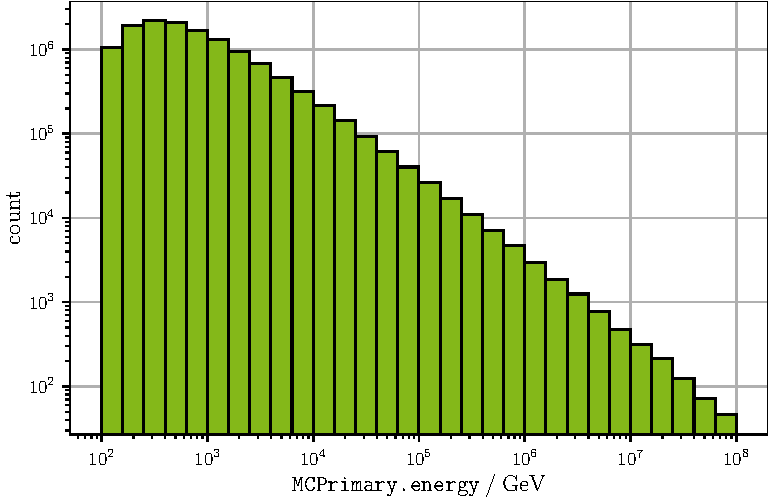
\includegraphics[scale=1]{content/plots/dataset:raw:histogram_full.pdf}
  \caption{Energy spectrum of the full, untouched Monte Carlo dataset using 30 bins.}
  \label{fig:dataset:raw:histogram}
\end{figure}


\clearpage
\section{Additional Hyperparameter Plots}
\begin{figure}
  \centering
  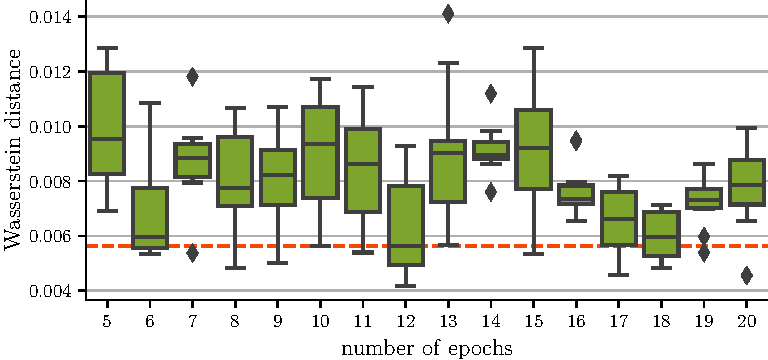
\includegraphics[scale=1]{content/plots/hyperparam/num_epochs_vs_wd_boxplot_lessheight.pdf}
  \caption{Boxplot of the accuracy for different epoch counts.}
  \label{fig:hyperparameter:num_epochs_vs_wd_boxplot}
\end{figure}

% COULDDO: add more?

\clearpage
\section{Bootstrap Distributions}
\begin{figure}
  \centering
  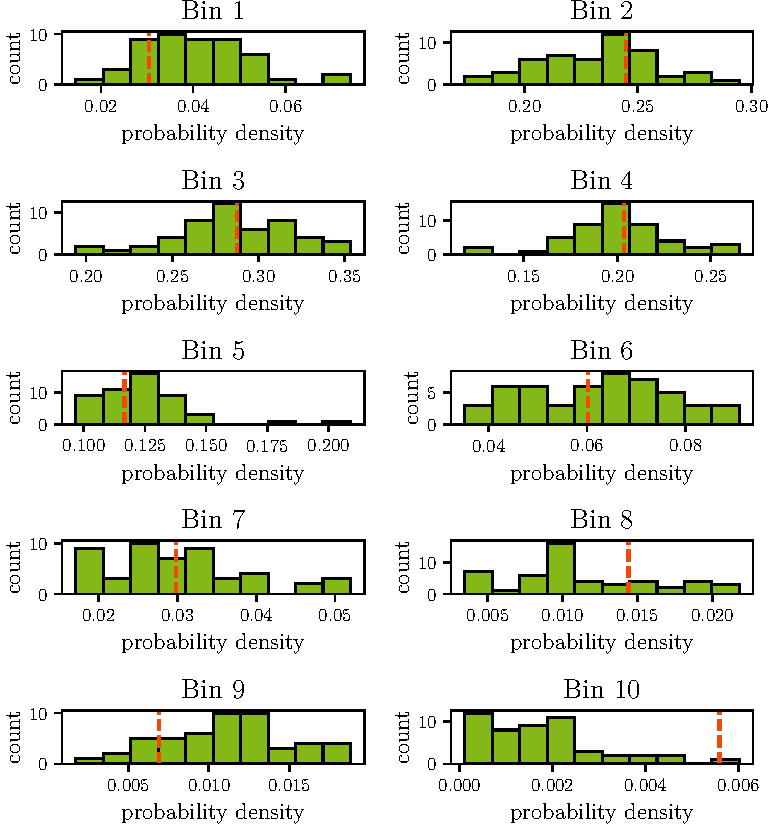
\includegraphics[scale=1]{content/plots/bootstrap:distributions_doubleheight.pdf}
  \caption{
    Bootstrap distributions of each bin in \autoref{fig:bootstrap:spectrum}.
    The dashed orange line shows the true value.
  }
  \label{fig:bootstrap:distributions}
\end{figure}


\clearpage
\section{Links etc.}
\begin{description}
  \item[Code on the chair's GitLab] \hfill \\
    \url{https://git.e5.physik.tu-dortmund.de/nweitkemper/Bachelor-code}
  \item[Dataset in the chair's \texttt{POOL} file system] \hfill \\
    \texttt{/net/big-tank/POOL/users/lkardum/new\_mc\_binning.csv} (\SI{14.6}{\giga\byte})
  % https://git.e5.physik.tu-dortmund.de/shaefs/bachelor_thesis/
\end{description}
